\subsection{Lista de funcionalidades}
\begin{frame}{Funcionalidades}
\begin{columns}[T]
	\begin{column}{.5\textwidth}
	\begin{itemize}
		\item Comercio electrónico
		\item Gestión de catálogo
		\item Gestión de precios y ofertas
		\item Gestión de usuarios
		\item Gestión de fabricación
		\item Gestión de encargos (compras y ventas)
		\item Gestión de contabilidad
		
	\end{itemize}
\end{column}
	\begin{column}{.5\textwidth}
	\begin{itemize}
		\justifying
		\item Empaquetado y envío
		\item Gestión de tareas, trabajos y proyectos
		\item Gestión de contenido (webs, blogs, foros o contenido general)
		\item Internacionalización y localización
	\end{itemize}
\end{column}
%Ref https://cwiki.apache.org/confluence/display/OFBIZ/OFBiz+Features#OFBizFeatures-BaseApplications
\end{columns}

\end{frame}

\begin{frame}
\begin{figure}[H]
	\centering
	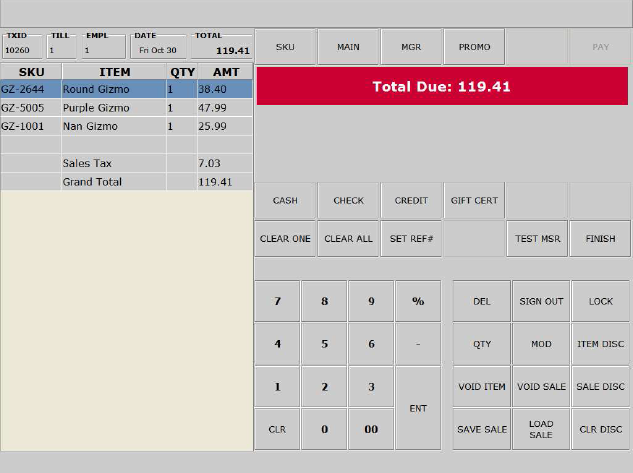
\includegraphics[width=0.9\linewidth]{img/posOfbiz.png}
	\caption{Captura de la funcionalidad Point Of Sales que ofrece Ofbiz, que es uno de los puntos más atractivos de este software}
	%Ref: https://cwiki.apache.org/confluence/display/OFBIZ/Information+on+translated+languages+in+OFBiz
\end{figure}

\end{frame}

\begin{frame}{Críticas a las funcionalidades}
\begin{columns}[T]
	
	\begin{column}{.5\textwidth}
		\justifying
		Algunas funcionalidades realmente necesarias, como la localización, están \textbf{incompletas}.
		\begin{figure}[H]
			\centering
			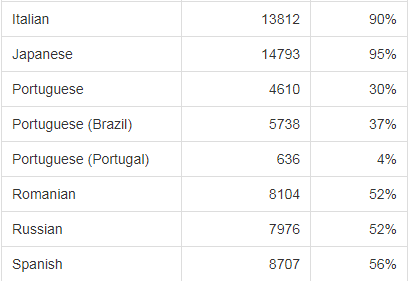
\includegraphics[width=0.8\linewidth, height=0.5\linewidth]{img/localisation.png}
			
		\end{figure}
		
		No hay funcionalidad para \textbf{contratación}, \textbf{tiempo de trabajo} ni \textbf{nómina}. 
	\end{column}
	\begin{column}{.5\textwidth}
		Faltan funcionalidades para \textbf{exportar} información, como por ejemplo PDFs o documentos de texto.
		\vspace{.5cm}
		
			
		\vspace{.5cm}
		
		Por último, no hay soporte directo para manejar el ERP desde \textbf{dispositivos móviles}, y se necesita software adicional para implementarlo.
	\end{column}
	
\end{columns}
	
\end{frame}

